\chapter{Automatización de canales BdB}
En este capítulo, se analizaró y modeló un proceso asignado por un colaborador del banco de Bogotá, el modelado del proceso se hará usando el estándar BPMN definido en el capítulo ~\ref{ch:BPMN}.


\section{Descripción del proceso (Automatización canales BdB)}
Desde área de Marketing y comunicaciones del banco de Bogotá surgió la iniciativa de automatizar el proceso de ``Canales'' donde las diferentes oficinas radican sus necesidades a las áreas de Publicidad y Mantenimiento, anteriormente las solicitudes que se le hacían al área de Marketing y comunicaciones se hacía por medio de correo electrónico y el seguimiento de estas se llevaba por medio de hojas de cálculo en Excel, la idea del área de marketing y comunicaciones es automatizar este proceso además de definir un canal por el cual las diferentes áreas puedan hacer sus solicitudes.\\

Para comenzar el proceso no lo puede iniciar cualquiera, el área de Marketing y comunicaciones recibe las solicitudes de los Jefes de oficinas, luego de que el Jefe de oficinas radique esta solicitud pasa a Client Partner Marketing el cual se encarga de validar las solicitudes que llegan al área, el tipo de solicitudes que llegan al área son las siguientes:\\
\begin{itemize}
	\item \textbf{Mantenimiento: } Los Jefes de oficina hacen estas solicitudes cuando  la pintura está dañada, una ventana rota, etc.
	\item \textbf{Otro: } Los Jefes de oficina seleccionan esta opción cuando piden una consulta (Referente a Marketing) o una recomendación.
	\item \textbf{Publicidad: }Los Jefes de oficina seleccionan esta opción cuando necesitan material publicitario como un afiche, tropezón, etc.
\end{itemize}

En caso de Mantenimiento Client Partner Marketing envía una notificación 
al Área administrativa y ellos se encargan del resto de la solicitud, cuando la solicitud es Otro, se le notifica al Comité de canales y ellos se encargan de gestionar la solicitud. En caso de Publicidad Client Partner Marketing asigna los estados de las solicitudes entrantes, entre las opciones que puede elegir están (Detenido, Cancelado y En progreso) donde cada estado define los siguientes pasos a ejecutar.
\begin{enumerate}
	\item Detenido: La solicitud se detiene y queda en este estado hasta que Cliente Partner Marketing le cambie el estado, una solicitud puede ser detenida por muchos factores, ejemplo la persona que hizo la solicitud se encuentra de vacaciones, etc.
	\item Cancelado: La solicitud se cancela y se le notifica al Jefe de oficinas que hizo la solicitud, las razones por la cuales se cancela la solicitud y se acaba el proceso.
	\item En progreso: La solicitud pasa de Client Partner Marketing a Client Partner Trade y se le notifica cuando esto sucede.
\end{enumerate}
En caso de la solicitud tener el estado de ``En progreso'' y haber notificado a Client Partner Trade, este gestiona y valida las solicitudes que le lleguen de Client Partner Markekting, también este puede cambiar el estado de las solicitudes entrantes puede elegir entre las opciones Detenido, Cancelado y En progreso, donde cada estado define los siguientes pasos a ejecutar:
\begin{enumerate}
	\item Detenido: La solicitud se detiene y queda en este estado hasta que Cliente Partner Trade le cambie el estado, una solicitud puede ser detenida por muchos factores, ejemplo la persona que hizo la solicitud se encuentra de vacaciones, etc.
	\item Cancelado: La solicitud se cancela y se le notifica a Client Partner Marketing porque se canceló y este a su vez al jefe de oficinas.
	\item En progreso: Se verifica si hay stock en bodega del material solicitado con Trade bodega.
\end{enumerate}

En caso de la solicitud tener el estado de ``En progreso'' y no tener stock en bodega, este le notifica a Client Partner Marketing y este a su vez al Jefe de oficinas y se cerraría el proceso.

En caso de haber stock se le envía una notificación al Jefe de oficinas con una fecha tentativa de entrega del material solicitado, también se le notifica a Client Partner Marketing que se va a realizar la entrega y también al analista de Trade, el analista de Trade debe alistar el material a enviar y notificar al proveedor de la entrega que se va a hacer, el proveedor le da una guía de seguimiento al analista de Trade y entrega el material a Client Partnert Marketing con un documento de entrega el Jefe de oficinas debe confirmar que recibió el material y notificar a Trade bodega para que este haga el cargue de documento de entrega y cerrar el proceso.\\

Modelo resultante (figura ~\ref{ABdB}).

\begin{figure}
	\centering
	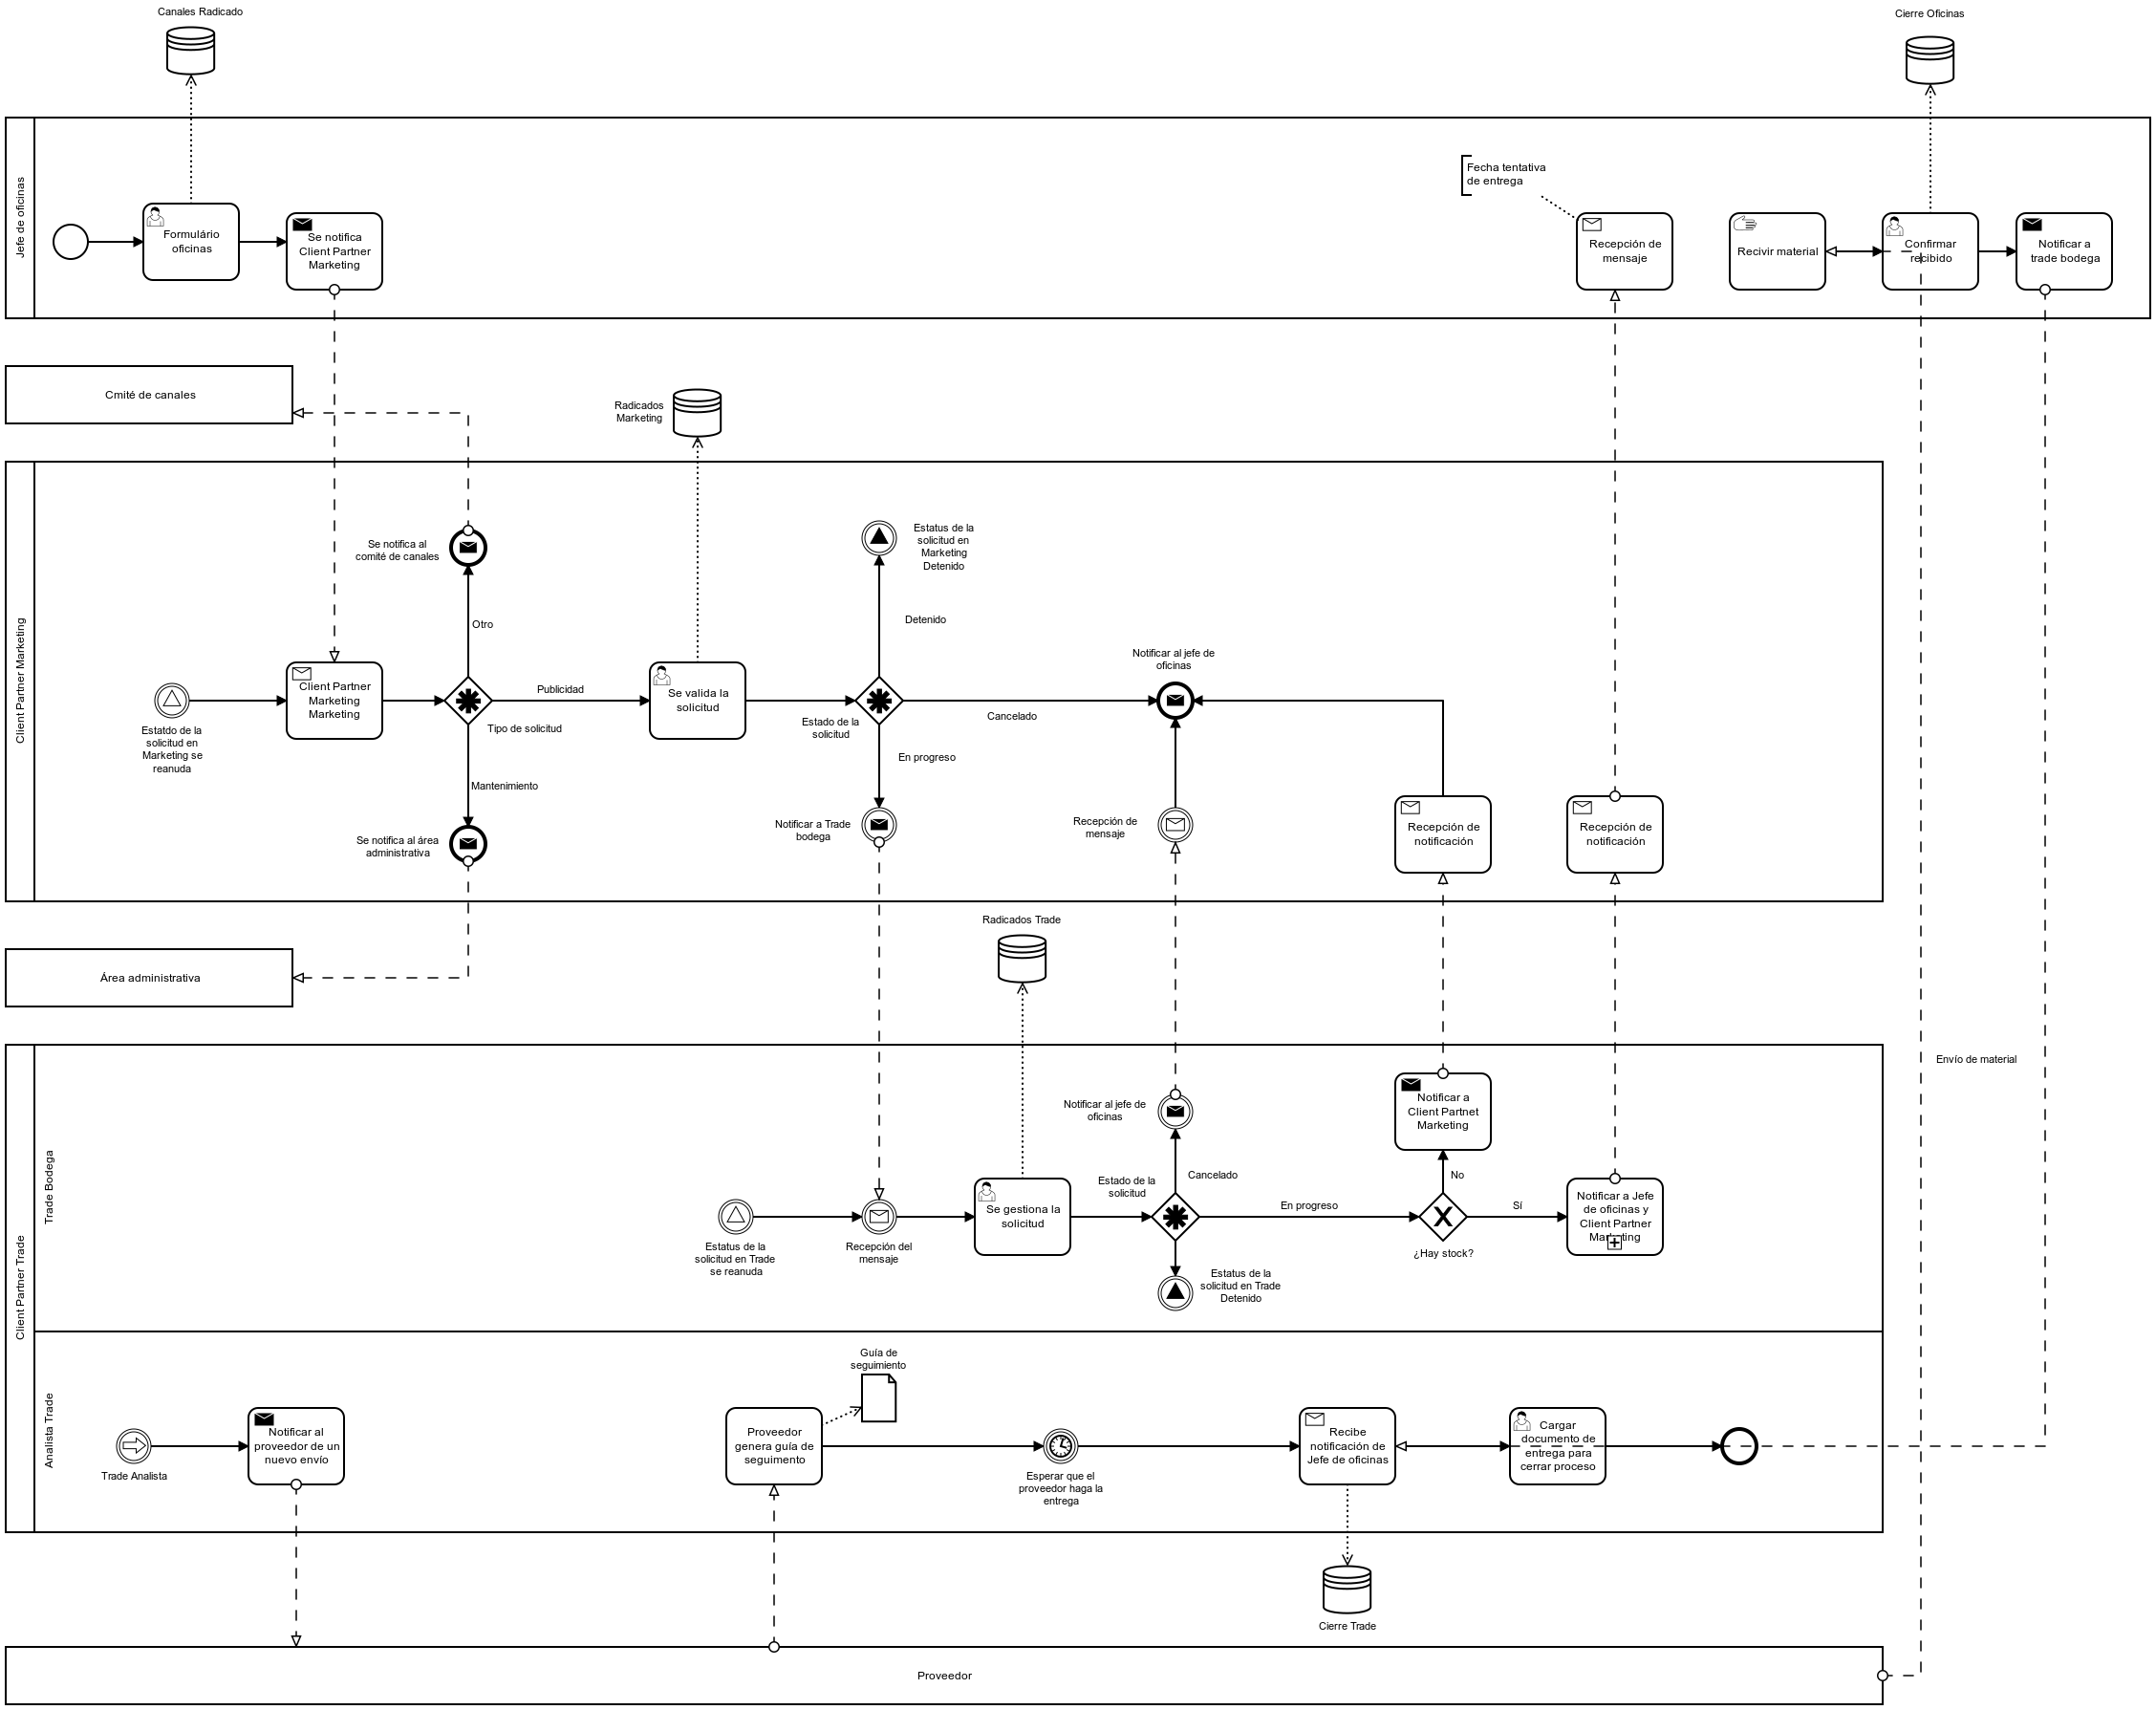
\includegraphics[scale=0.2]{Capitulo4/imagenes/diagram.png}
	\caption{Automatización de canales BdB }
	\label{ABdB}
\end{figure}

\section{Construcción del modelo}

\subsection{Participantes}
Dentro de la descripción podemos obtener los siguientes participantes: 
\begin{itemize}
	\item \textbf{Jefe de oficinas: }Es el colaborador que inicia el flujo al hacer la solicitud de publicidad, mantenimiento u otro.
	\item \textbf{Client Partner Marketing: } Colaborador de área de Marketing y comunicaciones que se encarga de gestionar todas las solicitudes entrantes.
	\item \textbf{Comite de canales: } Comité que al que se redirigen las solicitudes cuando es de tipo Otro, este participante es una ``Caja negra'' debido a que interactúa con el proceso, pero no hace parte del proceso.
	\item \textbf{Área administrativa: }Área a la que se redirigen las solicitudes de mantenimiento, este participante es una ``Caja negra'' debido a que interactúa con el proceso, pero no hace parte del proceso.
	\item \textbf{Client Partner Trade: }Área a la que se redirigen las solicitudes a las que Cliente Partner Marketing defina como ``En progeso''.
	\item \textbf{Proveedor: }Es un tercero un participante externo al proceso, pero con el que se interactúa, este participante es una ``Caja negra'' debido a que interactúa con el proceso, pero no hace parte del proceso.
\end{itemize}

Ya con los participantes identificados se da inicio al proceso usando un evento de inicio básico, el paso siguiente en el proceso es la radicación de un formulario por parte de un Jefe de oficinas, se usa una tarea de usuario para esta actividad, ya que el Jefe de oficinas debe ejecutar dicha tarea, en el formulario, el Jefe de oficinas tiene la opción de: 
\begin{enumerate}
	\item Radicar una solicitud de Mantenimiento, en dicha solicitud puede pedir, pintar una pared, arreglar un aviso, etc.
	\item Radicar una solicitud de Otro, en la cual puede hacer una consulta o pedir una recomendación.
	\item Radicar una solicitud de Publicidad, en la cual puede pedir materiales como afiches, tropezones, etc.
\end{enumerate}

\begin{figure}[H]
	\centering
	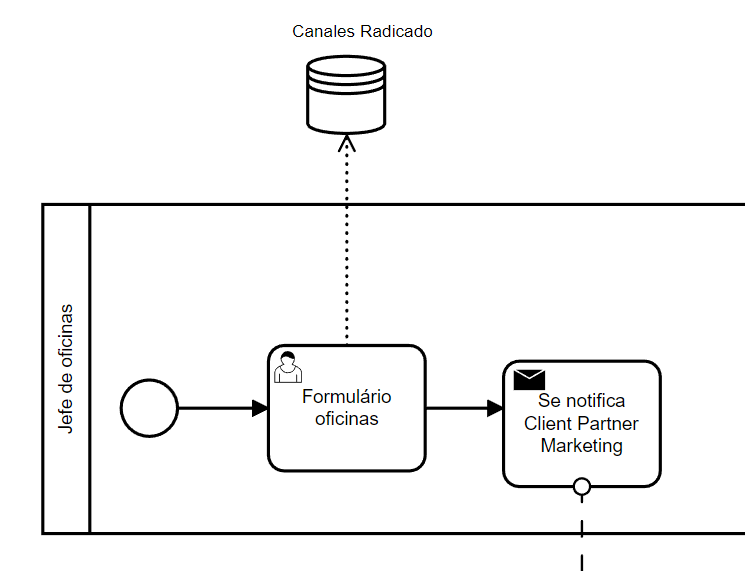
\includegraphics[scale=0.5]{Capitulo4/imagenes/1.png}
	\caption{Inicio del proceso}
	\label{inipro}
\end{figure}

Cuando un Jefe de oficinas radica la información se debe guardar para tener un historial y hacerle seguimiento a las distintas radicaciones que hacen los Jefes de oficina, luego de que el Jefe de oficinas haya hecho la solicitud, se evalúa el tipo de solicitud:
\begin{itemize}
	\item Si es de tipo Otro acaba el proceso, y se redirige la solicitud a comité de canales y ahí acaba el proceso.
	\item Si el proceso es de tipo Mantenimiento, se redirige la solicitud al área administrativa y ahí acaba el proceso.
	\item Si es de tipo Publicidad, pasa a Client Partner Marketing, el cual se encargará de darle trámite.
\end{itemize}

Dependiendo del tipo de solicitud que seleccione el Jefe de oficinas, el proceso se puede bifurcar en varios caminos, por esa razón se usó un Geteway Complejo. 

\begin{figure}[H]
	\centering
	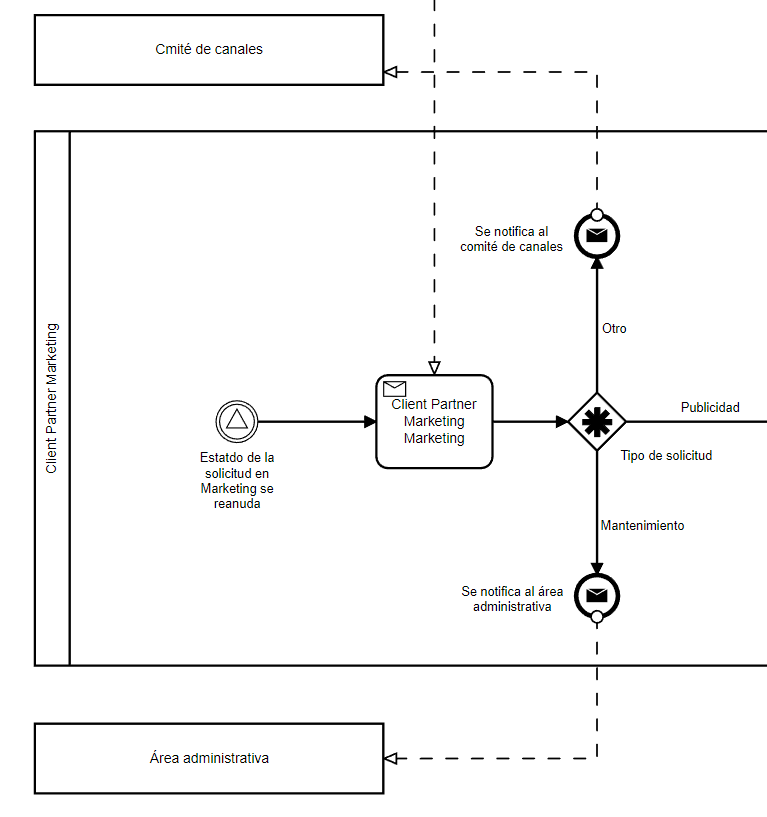
\includegraphics[scale=0.3]{Capitulo4/imagenes/3.png}
	\caption{Tipo de solicitud}
	\label{Tsol}
\end{figure}

Seguido, Client Partner Marketing debe validar la solicitud y definirle un estado a la solicitud, en este paso se ejecuta la tarea de usuario ``Se válida la solicitud'', los cambios que haga Client Partner Marketing y la información adicional que este agregue se guarda para tener un historial de las solicitudes que atiende y darle seguimiento a las mismas. Los estados que puede tomar una solicitud en el proceso son las siguientes: 
\begin{enumerate}
	\item Detenido: Cuando se selecciona este estado, la solicitud pasa a estado ``Detenido'' y queda a la esperando a que se le cambie el estado.
	\item Cancelado: Cuando se selecciona este estado se finaliza el proceso y se notifica al Jefe de oficinas.
	\item En progreso: Cuando se selecciona este estado, la solicitud se escala a Client Partner Trade.
\end{enumerate}
En este paso se usa un Gateway Complejo debido a que el proceso se puede bifurcar en varios caminos, dependiendo del camino que siga el proceso puede finalizarse o pasar a Client Partner Trade.
\begin{figure}[H]
	\centering
	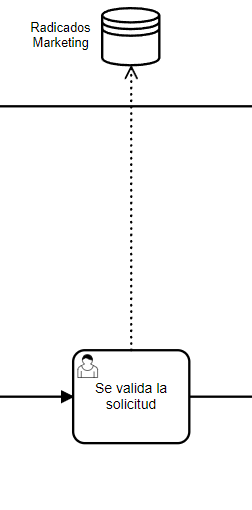
\includegraphics[scale=0.5]{Capitulo4/imagenes/11.png}
	\caption{Validación de solicitud}
	\label{ValSol}
\end{figure}


\begin{figure}[H]
	\centering
	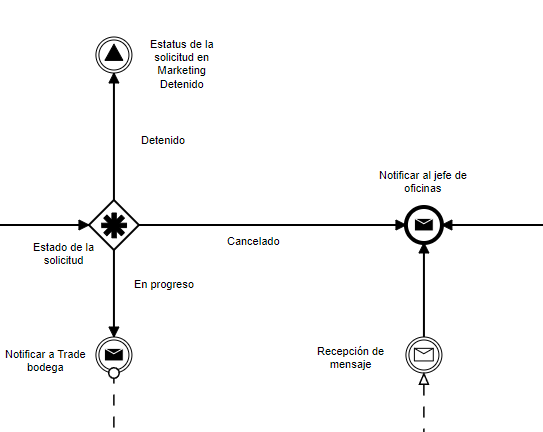
\includegraphics[scale=0.5]{Capitulo4/imagenes/5.png}
	\caption{Estado de solicitud}
	\label{Esol}
\end{figure}

El proceso continúa cuando Client Partner Marketing cambia el estado de la solicitud a ``En progreso'', cuando esto pasa se activa un evento intermedio de tipo Mensaje con el cual se notifica a Client Partner Trade que llegó una solicitud proveniente de Client Partner Marketing. Client Partner Trade recibe la notificación por parte de Client Partner Marketing y debe gestionarla aquí al igual que con Client Partner Marketing se debe guardar lo que gestione Client Partner Trade, en su gestión Client Partner Trade debe verificar que haya stock del material solicitado por eso el paso siguiente a gestionar la solicitud es un Gateway exclusivo donde se pregunta ¿Hay stock?, si la respuesta es no se debe notificar a Client Partner Marketing con una actividad de tipo Mensaje y este a su vez notifica al Jefe de oficinas que no hay stock y se finaliza el proceso.

\begin{figure}[H]
	\centering
	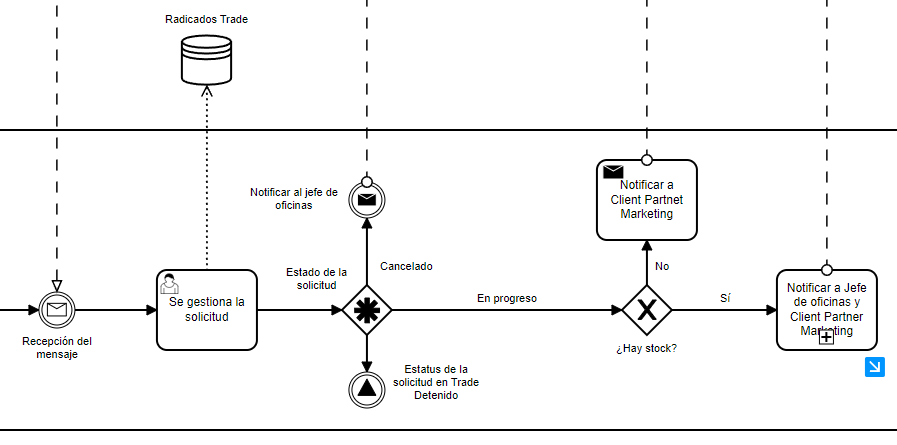
\includegraphics[scale=0.5]{Capitulo4/imagenes/6.png}
	\caption{Gestion Client Partner Trade}
	\label{Esol2}
\end{figure}

Cuando la respuesta es Si, continua un Subproceso el cual contiene las siguientes Tareas:
\begin{enumerate}
	\item Notificar al Jefe de oficinas una fecha tentativa de entrega.
	\item Notificar a Client Partner Marketing que la entrega se va a realizar.
	\item Notificar al analista de trade como debe cerrar el proceso y sigue un evento de tipo Link.
\end{enumerate}

\begin{figure}[H]
	\centering
	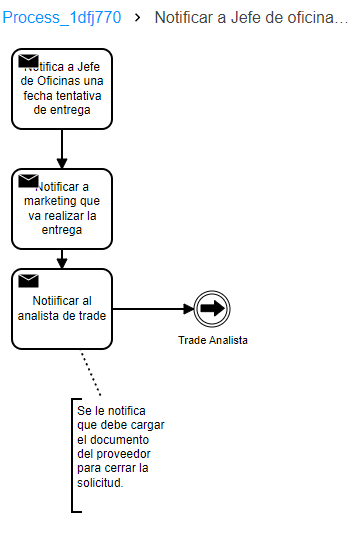
\includegraphics[scale=0.5]{Capitulo4/imagenes/7.png}
	\caption{SubProceso}
	\label{SubP}
\end{figure}

Luego de notificar Client Partner Marketing, también se le notifica al Jefe de oficinas que hizo la solicitud.

La última actividad del Subproceso activa el evento de tipo Link Trade Analista, el siguiente paso es notificar al proveedor de un nuevo envío que se debe hacer.

\begin{figure}[H]
	\centering
	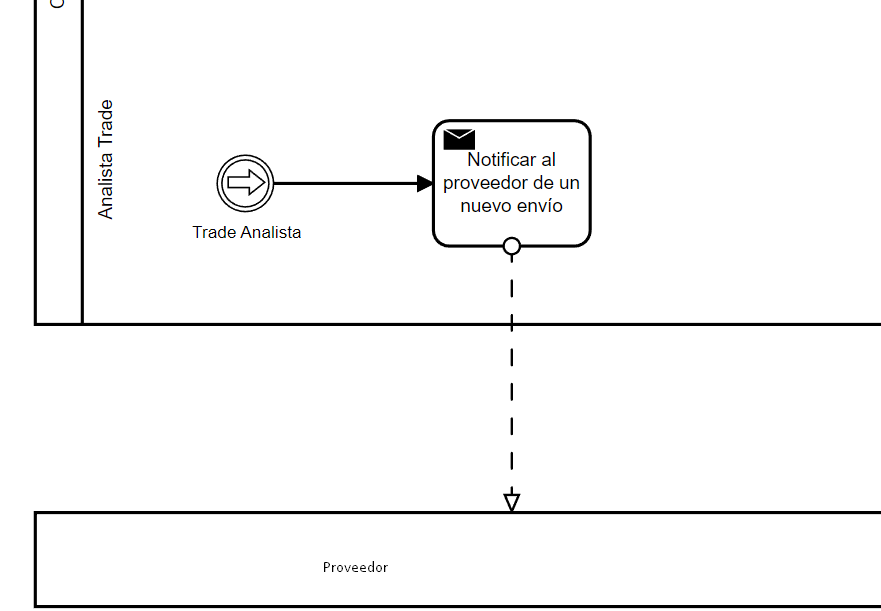
\includegraphics[scale=0.5]{Capitulo4/imagenes/8.png}
	\caption{Notificar a Proveedor}
	\label{SubP2}
\end{figure}

El proveedor como es un participante externo al proceso, pero que interactúa con él, el proveedor es el encargado de llevar a cabo el envío que solicite el analista de Trade, cuando el analista de Trade hace la solicitud de un envío al Proveedor, este le genera una guía de seguimiento (El proveedor es una distribuidora), luego se genera un evento intermedio de tipo Temporizador (Debe esperar que el proveedor haga la entrega del material), en este tiempo el proveedor debe hacer entrega del material.


\begin{figure}[H]
	\centering
	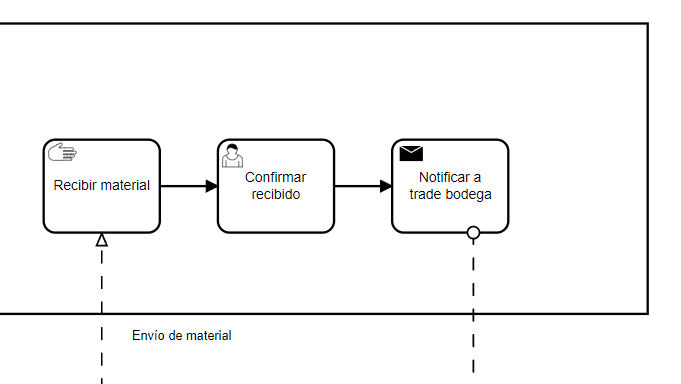
\includegraphics[scale=0.5]{Capitulo4/imagenes/9.png}
	\caption{Entrega del material}
	\label{Entregam}
\end{figure}

Cuando el Proveedor hace la entrega del material el Jefe de oficina debe recibirlo, por eso se define una actividad manual, seguido, debe confirmar en que recibió el material y notificar a Trade bodega, siguiendo el proceso, cuando Trade bodega recibe la notificación debe cargar la guía de seguimiento que genera el Proveedor y así finalizar el proceso.

\begin{figure}[H]
	\centering
	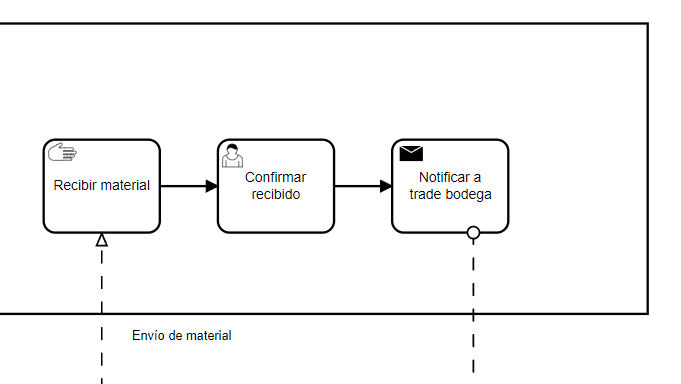
\includegraphics[scale=0.5]{Capitulo4/imagenes/9.png}
	\caption{Fin del proceso}
	\label{Finproc}
\end{figure}

\section{Implementación}
\subsection{Lista e SharePoint}\label{listasSp}
Las listas de SharePoint es la herramienta que se usa dentro de la organización para coleccionar y organizar datos que se usan o consumen los flujos de SharePoint y las aplicaciones de Power Apps, la estructura de la lista, así como los tipos de columna se hicieron acorde a la solicitud del colaborador de Marketing y comunicaciones.
\subsubsection{Lista Oficinas Marketing Canales}
\begin{figure}[H]
	\centering
	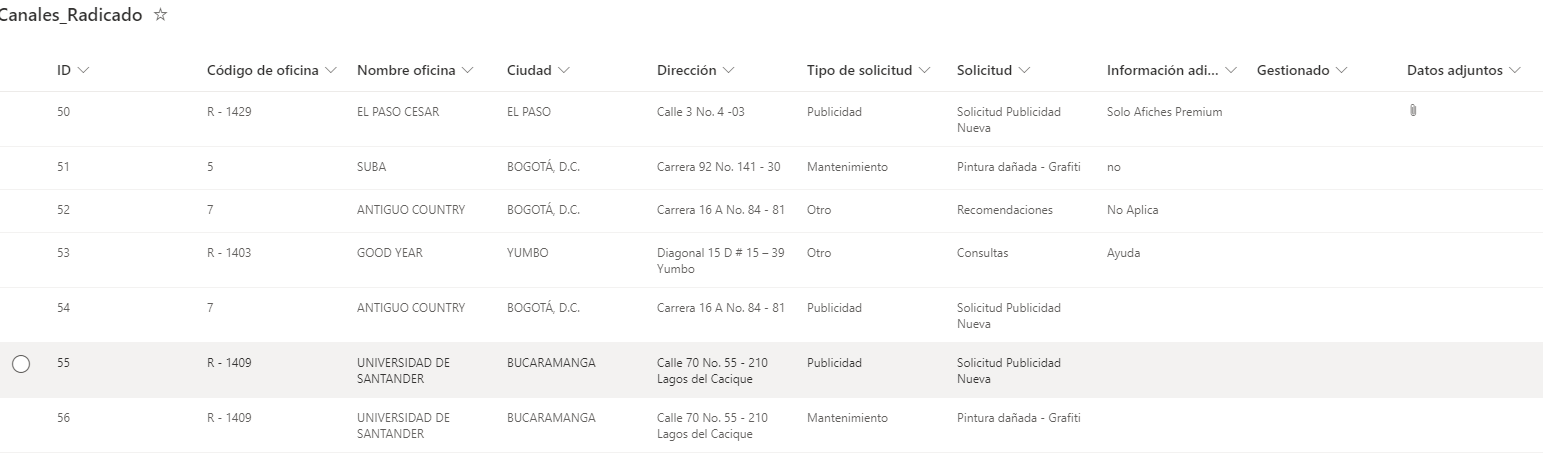
\includegraphics[scale=0.37]{Capitulo4/imagenes/12.png}
	\caption{Oficinas Marketing Canales}
	\label{OMC}
\end{figure}

\begin{figure}[H]
	\centering
	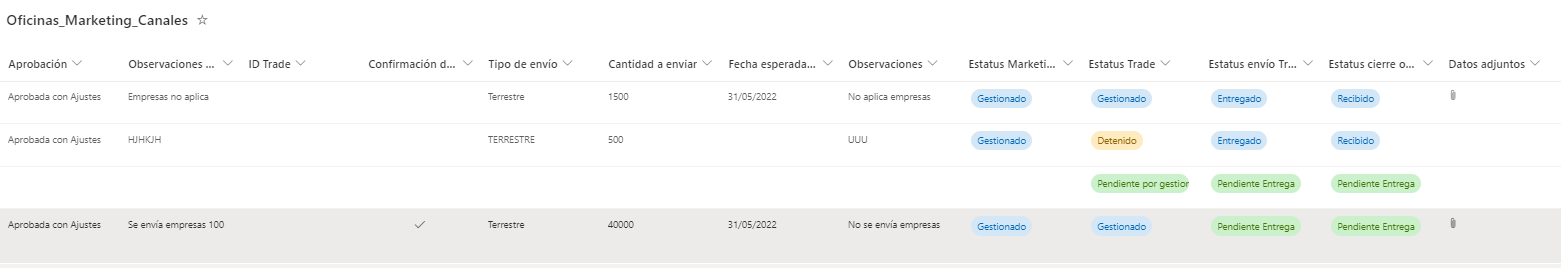
\includegraphics[scale=0.37]{Capitulo4/imagenes/13.png}
	\caption{Oficinas Marketing Canales}
	\label{OMC2}
\end{figure}

Las columnas se configuraron de la siguiente manera.

\begin{itemize}
	\item \textbf{ID: }Es una columna numérica única autoincrementable  que define SharePoint de manera automática.
	\item \textbf{ID Oficina: }Es una columna numérica que define las solicitudes hechas por los colaboradores del banco, esta columna se definió de tipo ``Número''.
	\item \textbf{Código de oficina: }Es un valor alfanumérico que tiene cada oficina y se utiliza para identificar de que oficina proviene una solicitud, por este motivo se define el tipo de la columna como ``Una sola línea de texto''.
	\item \textbf{ID Marketing: }Es una columna numérica que define las solicitudes atendidas por Client Partner Marketing, esta columna se definió de tipo ``Número''.
	\item \textbf{ID Marketing: }Es una columna numérica que define las solicitudes atendidas por Client Partner Marketing, esta columna se definió de tipo ``Número''.
	\item \textbf{Nombre oficina: }Es un valor alfabético o alfanumérico que define el nombre de una oficina, por este motivo se define el tipo de la columna como ``Una sola línea de texto''.
	\item \textbf{Ciudad: } Es un valor alfabético o alfanumérico que define el nombre de una oficina, por este motivo se define el tipo de la columna como ``Una sola línea de texto''.
	\item \textbf{Dirección: } Es un valor alfabético o alfanumérico que define el nombre de una oficina, por este motivo se define el tipo de la columna como ``Una sola línea de texto''.
	\item \textbf{Tipo de solicitud: } Es un valor de tipo alfabético, pero de un conjunto de valores permitidos (Publicidad, Mantenimiento u Otro), por este motivo se define el tipo de la columna como ``Opción''.
	\item \textbf{Solicitud: } Es un valor de tipo alfabético, por este motivo se define el tipo de la columna como `` Una sola línea de texto ''.
	\item \textbf{Información adicional: } Es un valor de tipo alfabético, pero debido a que el número de caracteres puede ser muy grande se define ``Varias líneas de texto'' debido a la capacidad que tienen de almacenar mayor cantidad de número de caracteres.
	\item \textbf{Estado de la solicitud: } Esta columna toma valores dependiendo de los estados que tenga la solicitud (En progreso, Cancelado, Detenido), esta columna se configuró de como ``Una sola linea de texto''.
	\item \textbf{Asignado a: } Esta columna almacenará obejeto con los atributos (Nombre, Email, Cargo, etc) del colaborador al cual se le asigne la solicitud, esta columna se configuró de tipo ``Usuario''.
	\item \textbf{Observaciones Marketing: } Tomará las observaciones que haga Client Partner Marketing, es un valor de tipo alfabético, pero debido a que el número de caracteres puede ser muy grande se define ``Varias líneas de texto'' debido a la capacidad que tienen de almacenar mayor cantidad de número de caracteres.
	\item \textbf{ID Trade: }Es una columna numérica que define las solicitudes atendidas por Client Partner Trade, esta columna se definió de tipo ``Número''.
	\item \textbf{Confirmación de inventario o stock de la solicitud: }Esta columna almacenará valores de tipo booleano (true o false), dependiendo si hay o no stock del material solicitado.
	\item \textbf{Tipo de envío: } Esta columna toma valores dependiendo del tipo de envío que se haga, esta columna se configuró de como ``Una sola linea de texto''.
	\item \textbf{Cantidad a enviar: }Es una columna numérica que define la cantidad de material a enviar por parte de Client Partner Trade, esta columna se definió de tipo ``Número''.
	\item \textbf{Datos adjuntos: } Es un tipo de datos complejo (Un objeto) donde se almacena el contenido del archivo, el nombre y la ruta donde está almacenado.
	\item \textbf{Observaciones Marketing: } Tomará las observaciones que haga Client Partner Marketing, es un valor de tipo alfabético, pero debido a que el número de caracteres puede ser muy grande se define ``Varias líneas de texto'' debido a la capacidad que tienen de almacenar mayor cantidad de número de caracteres.
	\item \textbf{Estatus Marketing: }Esta columna almacena una serie de valores permitidos (Gestionado, Pendiente por gestionar, Detenido, Rechazado, Cancelado) pero solo puede tomar uno de estos valores, esta columna se definió de tipo opción.
	\item \textbf{Estatus Trade: }Esta columna almacena una serie de valores permitidos (Gestionado, Pendiente por gestionar, Detenido, Rechazado, Cancelado) pero solo puede tomar uno de estos valores, esta columna se definió de tipo opción.
	\item \textbf{Estatus Envio Trade: }Esta columna almacena una serie de valores permitidos (Entregado, Pendiente Entrega, Sin inventario, Detenido, Rechazado, Cancelado) pero solo puede tomar uno de estos valores, esta columna se definió de tipo opción.
	\item \textbf{Estatus Cierre Oficinae: }Esta columna almacena una serie de valores permitidos (Recibido, Pendiente Entrega, Sin inventario, Detenido, Rechazado, Cancelado) pero solo puede tomar uno de estos valores, esta columna se definió de tipo opción.
\end{itemize}

\subsubsection{Lista de roles}
\begin{figure}[H]
	\centering
	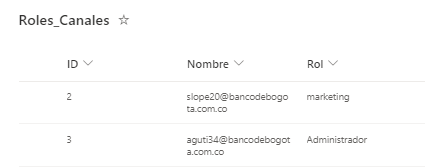
\includegraphics[scale=0.5]{Capitulo4/imagenes/17.png}
	\caption{Lista de Roles}
	\label{LRoles}
\end{figure}

\begin{itemize}
	\item \textbf{ID: }Es una columna numérica  único autoincrementable  que define SharePoint de manera automática.
	\item \textbf{Nombre: } En esta columna se almacenan valores de tipo alfanuméricos donde se guarda el correo de distintos colaboradores y su rol en la aplicación para controlar que puede o no ver o a que tiene acceso o no en la aplicación, se definió de ``Una sola línea de texto''.
	\item \textbf{Rol: }Es un valor alfanumérico que tiene cada colaborador y representa su rol dentro de la aplicación.
\end{itemize}


\subsection{Power Apps Studio}
La automatización podría funcionar perfectamente con la estructura de datos que se definió en la sección ~\ref{listasSp}, pero lo ideal es que los colaboradores no tengan que interactuar con las listas de SharePoint y tengan una experiencia más agradable en el proceso, para eso en Power Apps se crearon algunas pantallas en las cuales los colaboradores pueden hacer las solicitudes, hacerle seguimiento y cerrarlas.

\subsubsection{Pantallas}
Existe una pantalla de inicio donde dependiendo del Rol que tenga asignado puede ver o no ciertos controles dentro de la aplicación.

\begin{figure}[H]
	\centering
	
\includegraphics[scale=0.25]{Capitulo4/imagenes/18.png}
	\caption{Pantalla de inicio}
	\label{Pinicio}
\end{figure}

Ejemplo de la propiedad ``Visible'' en los bototones:

\begin{verbatim}
	If(
	LookUp(
	Roles_Canales;
	Nombre = Lower(varGlUser.Email)
	).Rol = "marketing" Or LookUp(
	Roles_Canales;
	Nombre = Lower(varGlUser.Email)
	).Rol = "Administrador";
	true;
	false
	)
\end{verbatim}

Se consulta el correo del usuario actual en la lista ``Roles\_Canales'' y pregunta si tiene el ``Marketing'' o ``Administrador'', si es cierto el resultado es ``true'' y el elemento (Seguimiento MArketing) es visible, de lo contrario se oculta.

\begin{figure}[H]
	\centering
	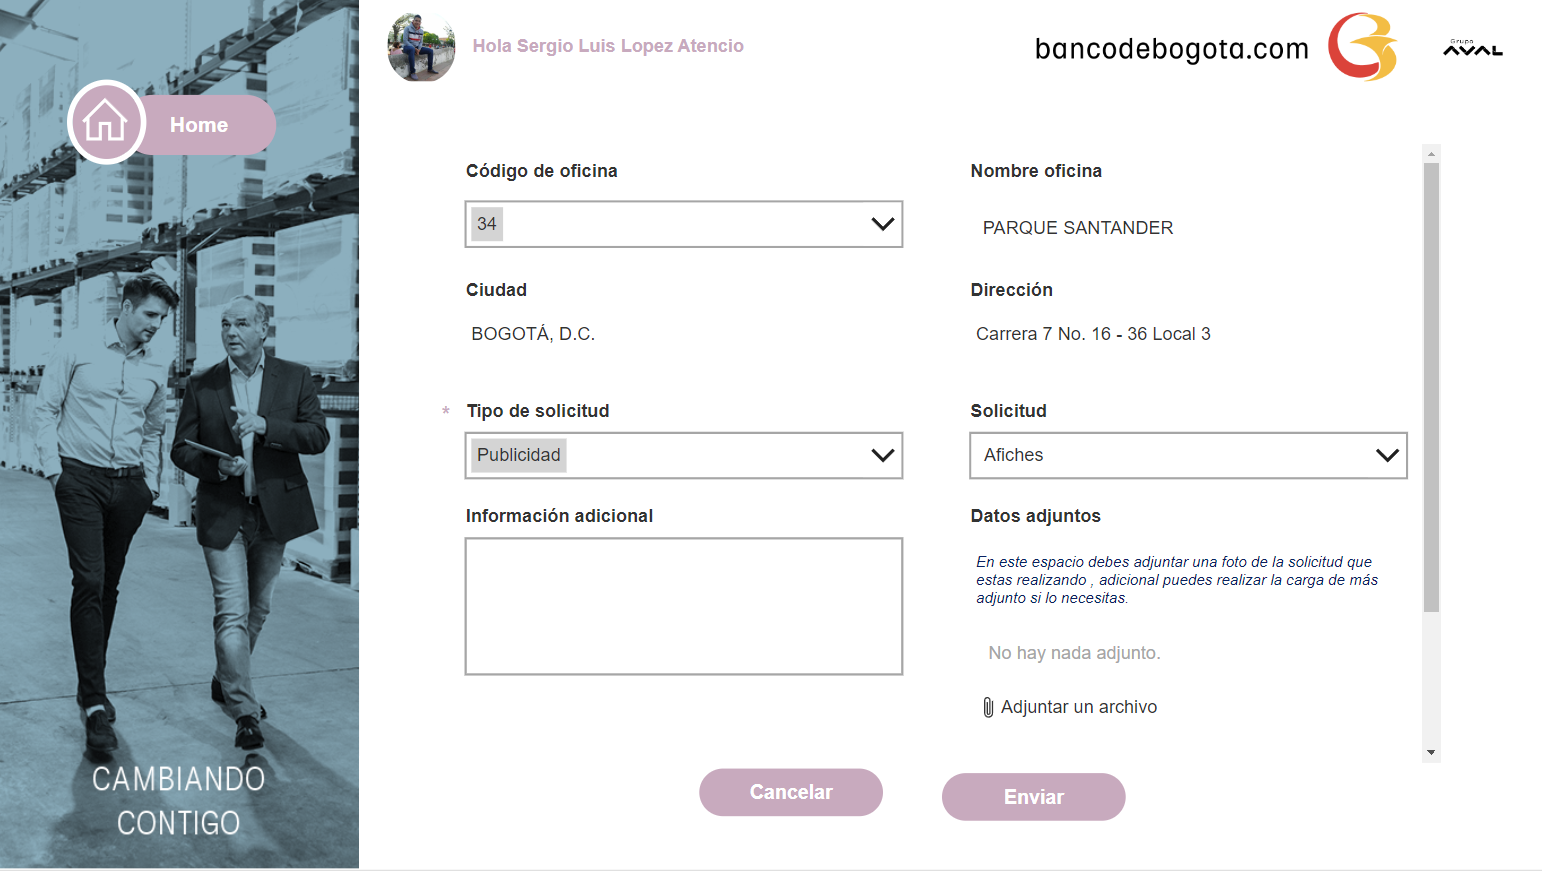
\includegraphics[scale=0.25]{Capitulo4/imagenes/19.png}
	\caption{Pantalla nueva solicitud}
	\label{Pform}
\end{figure}

Se hace uso de un formulario varios botones.
\begin{itemize}
	\item Home: Al presionarlo se devuelve a la pantalla de inicio.
	\begin{verbatim}
		Navigate(
		Screen_Solicitudes_Canales;
		ScreenTransition.Cover
		)
	\end{verbatim}
	\item Cancelar: Al presionarlo limpia el formulario y se devuelve a la pantalla de inicio.
	\item Enviar: Al presionarlo guarda el formulario en la lista Radicado Canales.
	\begin{verbatim}
		SubmitForm(Form_Radicado_Office)
	\end{verbatim}
\end{itemize}

\begin{figure}[H]
	\centering
	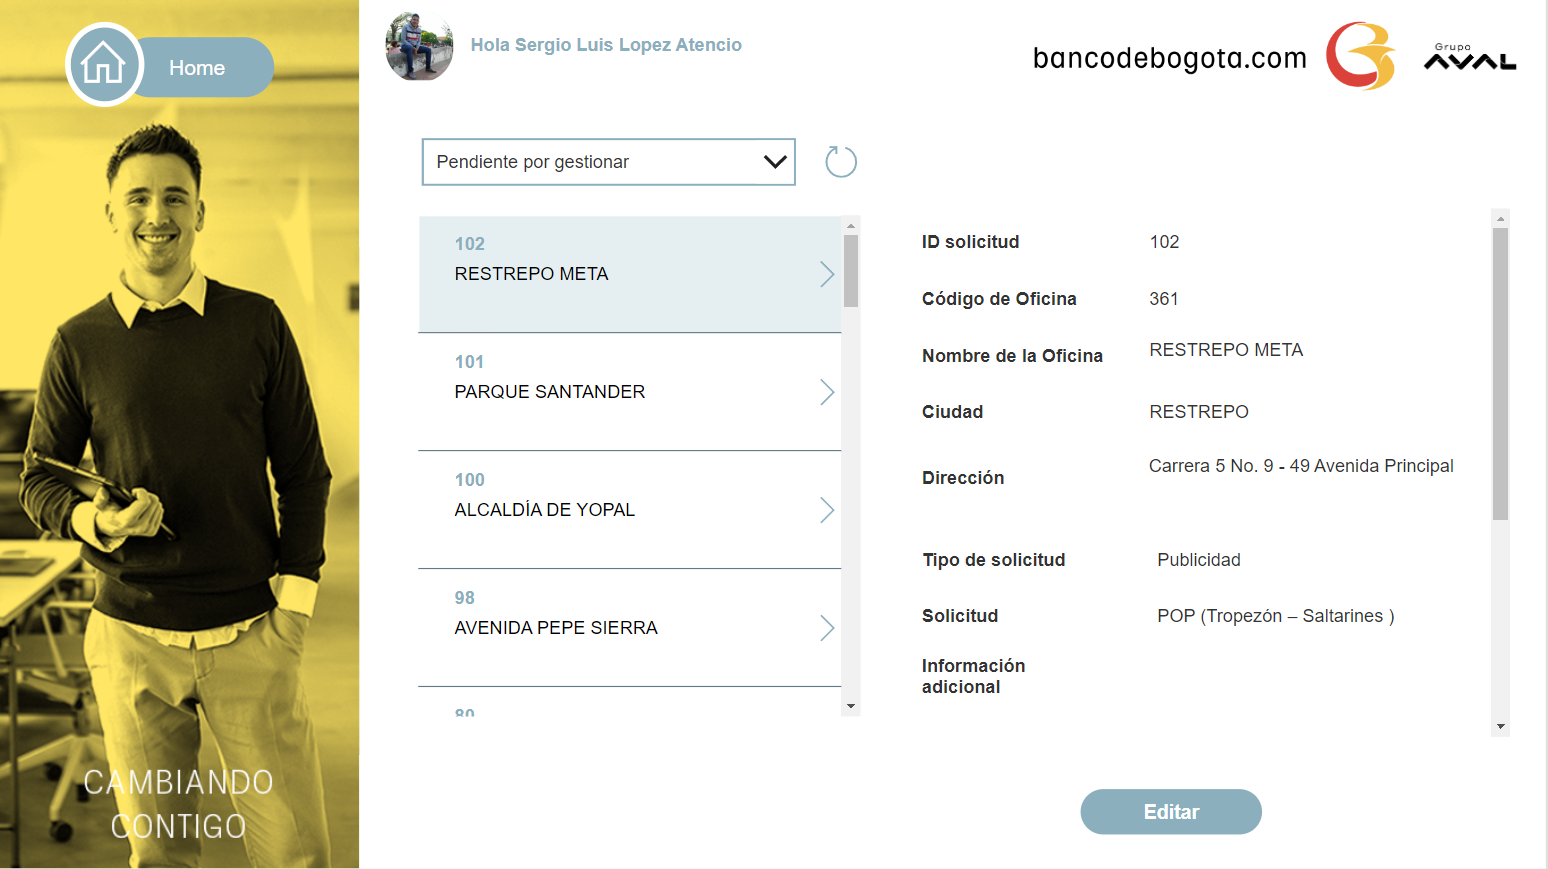
\includegraphics[scale=0.25]{Capitulo4/imagenes/20.png}
	\caption{Pantalla radicados canales}
	\label{PTotal}
\end{figure}

La galería se configuró de forma que organizara la información por la fecha en que se creó de manera descendente y se encuetre sin gestionar.
\begin{verbatim}
	Filter(
	Sort(
	Oficinas_Marketing_Canales;
	Creado;
	Descending
	);
	'Estatus Marketing'.Value = DropdownFiltroM.SelectedText.Value
	)
\end{verbatim}

El formulario de la derecha se configuró de manera que cambie de estado cuando Client Partner Marketing presine el botón editar.
\begin{verbatim}
	Filter(
	EditForm(Form_Radicado_Oficinas)
	)
\end{verbatim}

Cuando se presiona el icono de la flecha que apunta a la derecha muestre un formulario para gestionar la solicitud seleccionada en la galería.

\begin{figure}[H]
	\centering
	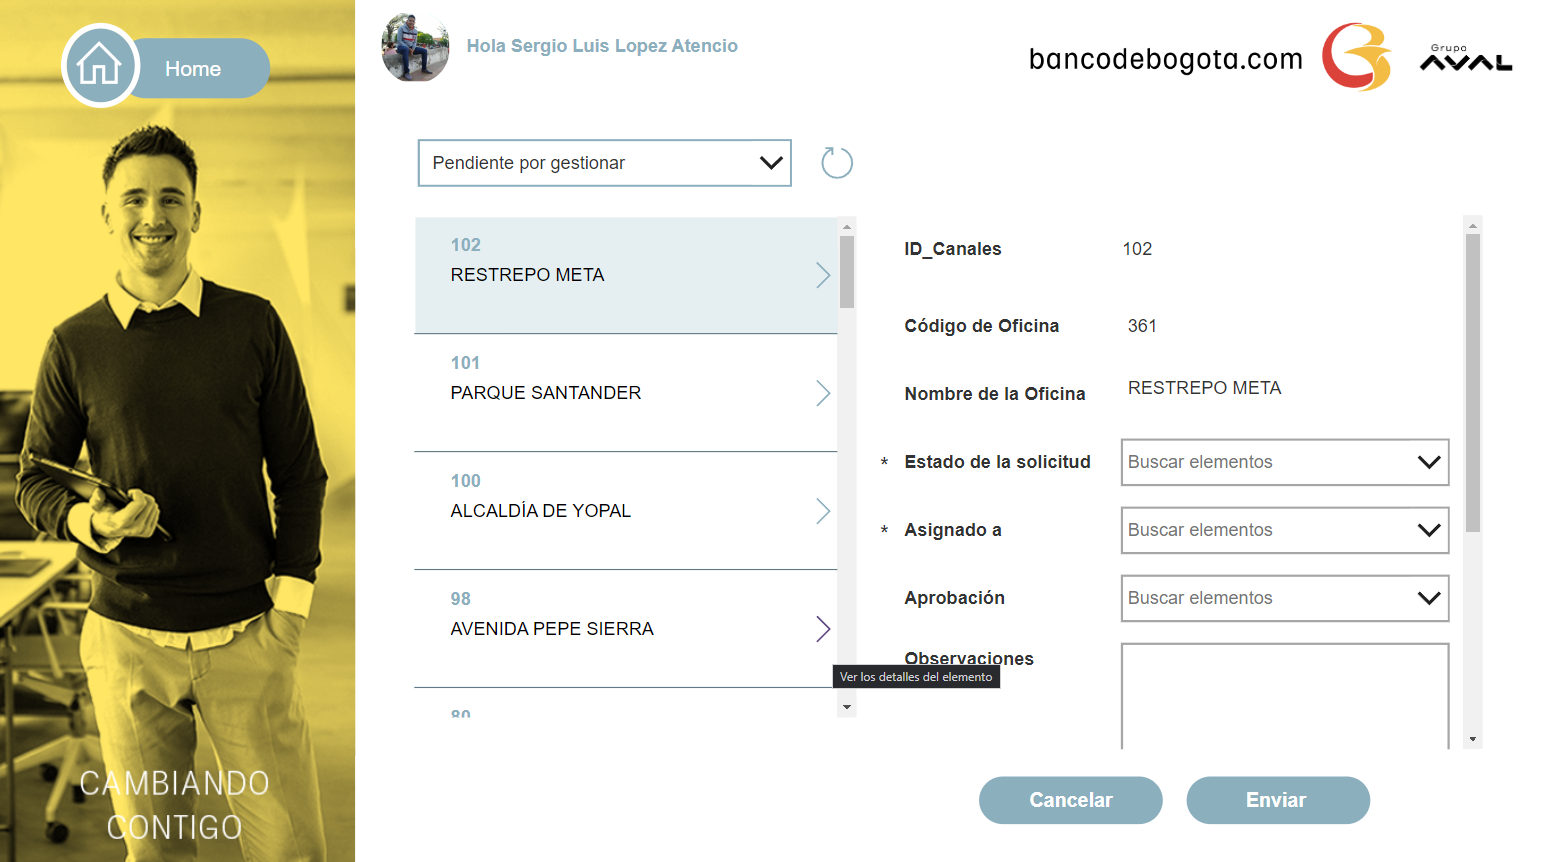
\includegraphics[scale=0.25]{Capitulo4/imagenes/21.png}
	\caption{Pantalla radicados canales}
	\label{PNMark}
\end{figure}

\begin{figure}[H]
	\centering
	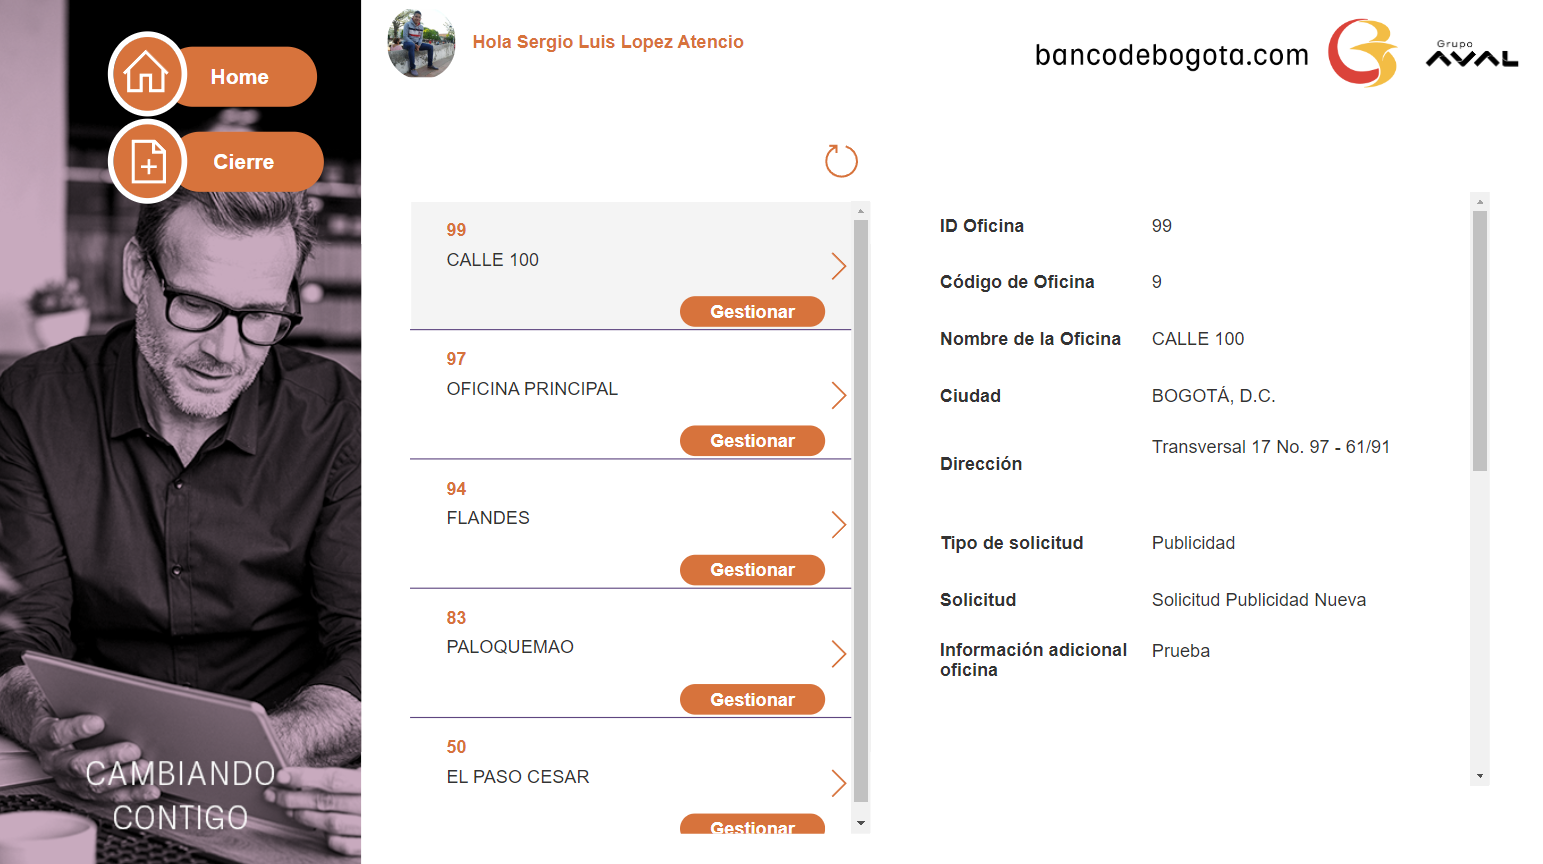
\includegraphics[scale=0.25]{Capitulo4/imagenes/22.png}
	\caption{Pantalla Trade}
	\label{PTrade}
\end{figure}


Esta pantalla muestra a Client Partner Trade las solicitudes que estén sin gestionar, haya gestionado Client Partner Marketing y sea de tipo Publicidad.

\begin{verbatim}
	Sort(
	Oficinas_Marketing_Canales;
	Creado;
	Descending
	);
	'Estatus Marketing'.Value = "Gestionado" And 'Tipo de solicitud'
	= "Publicidad" And 'Estatus Trade'.Value = "Pendiente por gestionar"
	)
\end{verbatim}

\begin{figure}[H]
	\centering
	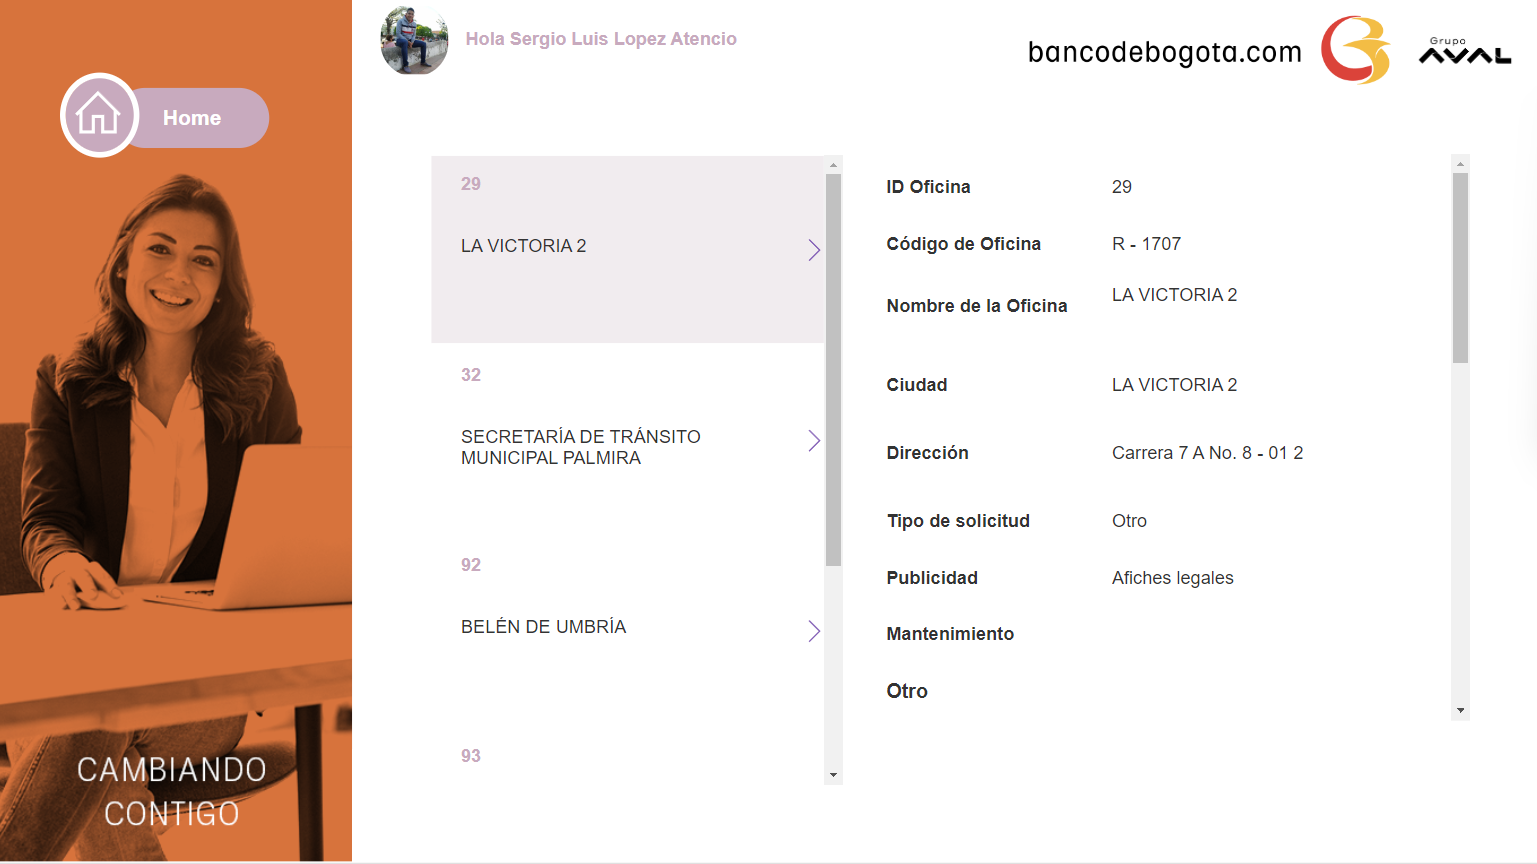
\includegraphics[scale=0.25]{Capitulo4/imagenes/23.png}
	\caption{Pantalla Cierre Oficina}
	\label{CTrea}
\end{figure}
En esta pantalla se mostrará todo lo que trade ha gestionado Client Partner Trade y el proceso esté listo para cerrar.


\begin{figure}[H]
	\centering
	
\includegraphics[scale=0.25]{Capitulo4/imagenes/24.png}
	\caption{Pantalla Cierre Oficina}
	\label{CTrea2}
\end{figure}

En esta pantalla mostrar todo lo que Client Partner Trade haya gestionado, en este paso se da el cierre del proceso cuando el analista de Trade recibe la notificación del Jefe de oficinas y sube el documento.